\chapter{Resultados adicionales de estimación de PLC}
\label{appendix_plc}

En este anexo se presentan los resultados complementarios de la estimación de PLC, discutidos en la sección \ref{sec:results_plc} del capítulo \ref{Chapter4}. Se incluyen el detalle del proceso de optimización de hiperparámetros, un análisis extendido del error en la predicción de DNBR y fracción de vacío (incluido el comportamiento del modelo fuera de la región de entrenamiento), los tiempos de cómputo obtenidos con la metodología propuesta y el análisis correspondiente al incorporar los embeddings de los perfiles de potencia.

\section{Optimización de hiperparámetros}
En la figura \ref{fig:plc_opt_results} se exponen los resultados durante el proceso de optimización del modelo de estimación de PLC.
\begin{figure}[H]
    \centering
    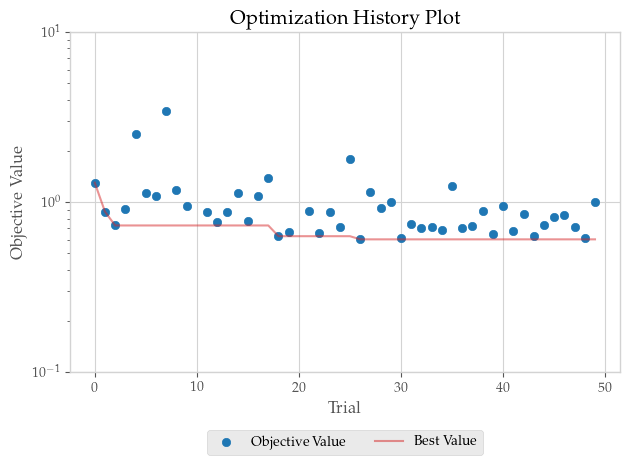
\includegraphics[width=0.7\textwidth]{Figures/plc_opt_result.png}
    \caption{Resultados de los distintos intentos de la optimización.}
    \label{fig:plc_opt_results}
\end{figure}

\section{Resultados de DNBR y fracción de vacío}
\label{sec:app_plc_dnbr_vacio}
Según la tabla \ref{tab:plc_errors_dnbr_vacio}, la tendencia general de la predicción de vacío es a sobrepredecir.
Por otro lado, el gráfico de predicho contra real de la figura \ref{fig:plc_results_dnbr_vacio} indica lo contrario. Para analizar esta discrepancia, se realizó el mismo cálculo del error al dividir en 5 regiones el dominio de cada variable objetivo. Los resultados se presentan en la tabla \ref{tab:plc_errors_dnbr_vacio_segmentado}. 

Por otro lado, para cuantificar el aumento del error en el conjunto excluido, la figura \ref{fig:plc_errores} presenta los errores para cada variable objetivo en los conjuntos de train, test y excluidos. Tal como se comentó previamente, los conjuntos de train y test presentan errores muy similares, y el conjunto excluido un error considerablemente mayor. Adicionalmente, se grafican los cuantiles del 5\% y 95\%, que evidencian que el conjunto de excluidos también tiene una dispersión mucho mayor en su error.

\begin{table}[h]
	\centering
	\caption{Media y desvío estándar del error con signo para cada objetivo, segmentado por rangos de cada objetivo.}
	\begin{tabular}{c c c c c c} 
        \toprule
        \multirow{3}{1.5cm}{\textbf{Objetivo}} & \multirow{3}{*}{\textbf{Rango}} & \multicolumn{4}{c}{\textbf{Conjunto}} \\
        &                                               & \multicolumn{2}{c}{Train} & \multicolumn{2}{c}{Test} \\ 
        &                                               & media & $\sigma$  & media & $\sigma$  \\
        \multirow{5}{1.5cm}{DNBR}               
                        &$   <1.7$  & $0.003$ &   $0.004$   & $0.000$ &  $0.008$    \\ 
                        &$1.7-2.5$  & $-0.001$&   $0.009$   & $-0.001$&  $0.013$    \\
                        &$2.5-3.5$  & $-0.013$&   $0.013$   & $-0.015$&  $0.019$    \\
                        &$  3.5-5$  & $-0.044$&   $0.038$   & $-0.042$&  $0.051$    \\
                        &$     >5$  & $-0.051$&   $0.039$   & $-0.015$&  $0.076$    \\
        \hline
        \multirow{5}{1.5cm}{Fracción de vacío}
                        &$        0$  & $-0.035$ & $0.033$ & $0.061$ & $0.037$ \\ 
                        &$   0-0.15$  &  $0.013$ & $0.021$ & $0.010$ & $0.032$ \\
                        &$0.15-0.35$  &  $0.024$ & $0.036$ & $0.025$ & $0.044$ \\
                        &$ 0.35-0.6$  &  $0.007$ & $0.021$ & $0.007$ & $0.027$ \\
                        &$     >0.6$  &  $0.031$ & $0.022$ & $0.024$ & $0.014$ \\

		\bottomrule
	\end{tabular}
	\label{tab:plc_errors_dnbr_vacio_segmentado}
\end{table}

\begin{figure}[h]
    \centering
    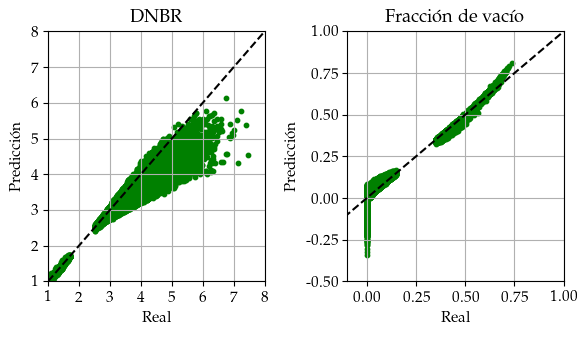
\includegraphics[width=0.7\textwidth]{Figures/plc_pred_excluidos.png}
    \caption{Resultados de predicción de DNBR y fracción de vacío, para el conjunto excluido.}
    \label{fig:plc_results_excluidos}
\end{figure}

\begin{figure}[H]
    \centering
    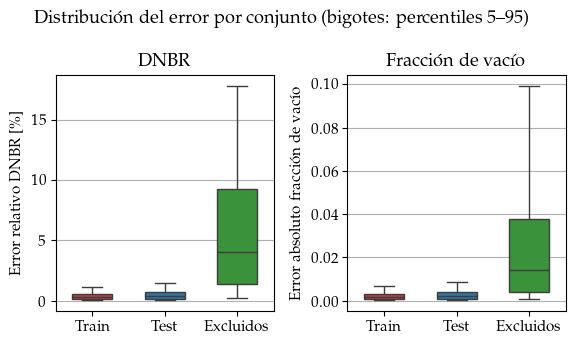
\includegraphics[width=0.7\textwidth]{Figures/plc_error.png}
    \caption{Distribución del error para cada objetivo, por conjunto de datos.}
    \label{fig:plc_errores}
\end{figure}

\section{Tiempos de cómputo de la estimación de PLC}
\label{app_plc_tiempos}
En la tabla \ref{tab:plc_tiempos} se presenta un resumen de los tiempos de cómputo para el cálculo de PLC. Los resultados son contundentes: la mejora o speedup del proceso de cálculo alcanza una media de entre $8\,409$ y $9\,519$ para DNBR, y de entre $2\,197$ y $2\,486$ para fracción de vacío. El tiempo total de cómputo pasó de las 380 h con COBRA3-CP a alrededor de 4 minutos con la DNN. Esto sustenta el valor de este modelo, que no solo logra una predicción de las PLC con un error acotado, sino que además requiere un tiempo de cómputo varios órdenes de magnitud inferior. Por otra parte, no se implementaron lógicas adicionales para lograr un cómputo más eficiente por medio de la DNN, como el procesamiento en batch. Se computaron todos los casos en serie, tanto en CPU como en GPU. Estos aspectos representan oportunidades de mejora, como se explica en el capítulo \ref{Chapter5}.

\begin{table}[H]
	\centering
	\caption{Tiempos de cómputo para cálculo de PLC.}
	\begin{tabular}{l l c c c c c} 
        \toprule
        & & \multicolumn{3}{c}{\textbf{Tiempo}} & \multicolumn{2}{c}{\multirow{2}{*}{\textbf{Mejora}}} \\
        & & \multirow{2}{*}{\textbf{COBRA3-CP [s]}} & \multicolumn{2}{c}{\textbf{DNN [ms]}} &  \\
        & &                                     & CPU & GPU & CPU & GPU \\
        \hline
        \multirow{4}{1.5cm}{DNBR}   
                                & mínimo        & $8.53$      & $0.28$  & $0.47$ & 3 562   & 406 \\
                                & media         & $25.16$     & $2.66$  & $3.03$ & 9 519   & 8 409\\
                                & máximo        & $137.95$    & $5.88$  & $5.51$ & 57 882 & 48 363\\
                                & \textbf{total}& 306 h     & 117 s & 130 s& 9 445  & 8 503\\
        \hline
        \multirow{4}{1.5cm}{Fracción de vacío}  
                                & mínimo        & $1.07$      & $0.21$  & $0.33$  & 432   & 405\\
                                & media         & $6.09$      & $2.46$  & $2.80$  & 2 486  & 2 197\\
                                & máximo        & $14.70$     & $5.70$  & $6.69$  & 5 955  & 5 385\\
                                & \textbf{total}& 74 h     & 108 s & 120 s & 2 479  & 2 224\\
		\bottomrule
	\end{tabular}
	\label{tab:plc_tiempos}
\end{table}


\section{Análisis del error en la aplicación de embeddings}
\label{app_plc_emb_errores}
Una vez entrenado el encoder, se evaluó la arquitectura del predictor de PLC, pero con el espacio latente de los perfiles de potencia como entradas. Se plantearon tres modelos, que utilizan el espacio latente del perfil axial, el del perfil por barras y ambos espacios latentes. En la tabla \ref{tab:plc_emb_errors_dnbr_vacio} se presentan la media y el desvío estándar del error con signo, para los tres modelos con embeddings y el modelo base. Los tres modelos presentan una reducción de la media del error en ambas variables objetivo. En cuanto al desvío estándar, para DNBR no se obtiene una reducción significativa, pero para fracción de vacío se reduce a aproximadamente la mitad. Es importante señalar que los modelos con embeddings del perfil por barras y de ambos perfiles presentan una media positiva del error de DNBR. Por otro lado, los tres modelos presentan un error medio negativo para la fracción de vacío. Estos dos puntos son un resultado no conservativo, aunque no de forma excesiva.

\begin{table}[h]
	\centering
	\caption{Media y desvío estándar del error con signo para cada objetivo, para modelos con embeddings.}
	\begin{tabular}{l c c c c c} 
        \toprule
        \multirow{2}{*}{\textbf{Modelo}} & \multirow{2}{*}{\textbf{Conjunto}} & \multicolumn{2}{c}{\textbf{DNBR}} & \multicolumn{2}{c}{\textbf{Fracción de vacío}} \\
        &         & media     & $\sigma$  & media & $\sigma$  \\ \hline
        \multirow{2}{*}{Base}
        & Train   &  $-0.006$    & $0.021$     & $0.018$ & $0.040$ \\
        & Test    &  $-0.006$    & $0.017$     & $0.018$ & $0.032$ \\ \hline
        \multirow{2}{*}{Emb. perfil axial}
        & Train   & $-0.002$ & $0.018$ & $-0.002$ & $0.021$ \\
        & Test    & $-0.001$ & $0.020$ & $-0.002$ & $0.022$   \\   \hline
        \multirow{2}{*}{Emb. perfil por barras}
        & Train   & $0.001$ & $0.013$ & $-0.006$ & $0.021$ \\
        & Test    & $0.001$ & $0.014$ & $-0.006$ & $0.022$ \\   \hline
        \multirow{2}{*}{Emb. ambos perfiles}
        & Train   & $0.000$ & $0.017$ & $-0.011$ & $0.016$ \\
        & Test    & $0.000$ & $0.020$ & $-0.010$ & $0.017$ \\

		\bottomrule
	\end{tabular}
	\label{tab:plc_emb_errors_dnbr_vacio}
\end{table}

\chapter{Resultados adicionales de estimación de CHF}
\label{appendix_chf}

En este anexo se presentan los resultados complementarios de la estimación de CHF, discutidos en la sección \ref{sec:results_chf} del capítulo \ref{Chapter4}. Se incluyen el detalle del modelo predictor de CHF en un tubo, tanto en su versión \lfdnn{} como en la versión informada por física \lfpinn{}; el análisis de arquitectura informada por física para las variantes evaluadas del modelo \mfpinn{}; el análisis de las variables de entrada adicionales consideradas para el modelo; y los resultados del modelo final \mfdnn{}.

\section{Modelo predictor de CHF en un tubo}
\label{app_chf_lfdnn_resultados}
Como se comentó en la sección \ref{sec:chf_arq}, se construyó un modelo de DNN para predecir el CHF en un tubo. Esta red se utiliza luego como entrada de las \mfdnn{} y \mfpinn{} entrenadas. Es importante notar que, para que los modelos de multifidelidad obtengan información relevante de la estimación en un tubo, esta debe ser confiable y tener valor físico. Por ello, la evaluación de la \texttt{LFDNN} entrenada no se restringe únicamente a estadísticos tradicionales. Para su evaluación se consideran tres categorías principales: su predicción de los ensayos en un tubo, su $\mathrm{DNBR}_\mathrm{min}$ derivado de sus predicciones sobre los ensayos de la Universidad de Columbia y la evolución del CHF predicho en función de los parámetros termohidráulicos. Este último criterio se propuso debido a que redes con arquitecturas muy densas y profundas lograban muy buenos resultados en los primeros dos criterios, pero al mirar en detalle la relación del CHF con los parámetros termohidráulicos se observaban tendencias no físicas.

Entonces, para encontrar una arquitectura óptima resultaba difícil recurrir a una estructura automatizada como Optuna. Se propuso, en cambio, analizar una serie limitada de arquitecturas, para evaluar el impacto del ancho y la profundidad de la red en los resultados. En la tabla \ref{tab:lfdnn_arqs} se presentan las arquitecturas evaluadas y sus métricas estadísticas. Se evaluó utilizar como función de activación la tangente hiperbólica y la función SiLU. Finalmente, la función SiLU fue la que demostró un comportamiento más estable.
Se observa que todos los modelos logran tanto en entrenamiento como en evaluación un $\mathrm{R}^2>0.95$ y un RMSE menor a $400\,\mathrm{kW/m^2}$. Los modelos con menos parámetros presentan una menor diferencia entre el RMSE del conjunto de entrenamiento y el de evaluación. Los dos modelos con mayor cantidad de parámetros presentan los mejores valores tanto de $\mathrm{R}^2$ como de RMSE. En vista de estos resultados, se podría considerar que el entrenamiento de todas las redes es satisfactorio.

\begin{table}[h]
	\centering
	\caption{Arquitecturas de \texttt{LFDNN} propuestas y métricas sobre conjuntos de entrenamiento y evaluación de ensayos en un tubo.}
	\begin{tabular}{c C{2cm} C{2cm} c c c c} 
        \toprule
        \multirow{2}{*}{\textbf{\#}} & \multirow{2}{=}{\textbf{Dim. capas ocultas}} & \multirow{2}{=}{\textbf{Cant. capas ocultas}} & \multicolumn{2}{c}{$\mathbf{R^2}$} & \multicolumn{2}{c}{\textbf{RMSE}} \\
        & & & \textbf{Ent.} & \textbf{Eval.} & \textbf{Ent.} & \textbf{Eval.} \\ \hline
        \multicolumn{3}{c}{LUT}   & \multicolumn{2}{c}{$0.898$} & \multicolumn{2}{c}{$507.1$} \\
        1 & 64  & 2 & $0.9553$ & $0.9590$ & $337.9$ & $322.0$ ($+0.8\%$) \\
        2 & 64  & 3 & $0.9657$ & $0.9657$ & $296.1$ & $294.3$ ($+4.2\%$) \\
        3 & 64  & 4 & $0.9749$ & $0.9738$ & $253.0$ & $257.3$ ($+14.2\%$) \\
        4 & 32  & 3 & $0.9503$ & $0.9557$ & $356.0$ & $334.6$ ($+0.3\%$) \\
        5 & 128 & 3 & $0.9746$ & $0.9753$ & $254.9$ & $249.9$ ($+9.6\%$) \\
		\bottomrule
	\end{tabular}
	\label{tab:lfdnn_arqs}
\end{table}
% Groeneveld  |            log CHF            |          CHF [kW/m2]          
% modelo       R2 tr   R2 te  RMSE tr  RMSE te   R2 tr   R2 te   RMSE tr   RMSE te
% ------------------------------------------------------------------------------
% 64x2        0.9608  0.9599   0.1583   0.1595  0.9553  0.9590     337.9     322.0
% 64x3        0.9683  0.9653   0.1425   0.1484  0.9657  0.9657     296.1     294.3
% 64x4        0.9778  0.9709   0.1192   0.1361  0.9749  0.9738     253.0     257.3
% 32x3        0.9600  0.9595   0.1600   0.1605  0.9503  0.9557     356.0     334.6
% 128x3       0.9754  0.9702   0.1254   0.1375  0.9746  0.9753     254.9     249.9

% mejor R2 en test (log):   64x4  (0.9709)
% mejor RMSE en test (log): 64x4  (0.1361)

% brecha train->test (RMSE en log):
%   64x2       +0.0012 (+0.8%)
%   64x3       +0.0059 (+4.2%)
%   64x4       +0.0169 (+14.2%)
%   32x3       +0.0005 (+0.3%)
%   128x3      +0.0121 (+9.6%)

En la tabla \ref{tab:lfdnn_dnbrmin} se presentan los resultados de las distintas arquitecturas al evaluar sobre el conjunto de datos de los ensayos de Columbia replicados con COBRA3-CP. Se presentan la media y el desvío estándar del $\mathrm{DNBR}$ predicho y el $\mathrm{DNBR}_\mathrm{min}$. Adicionalmente, se calcularon cuántos casos de los 146 presentaron el valor mínimo de CHF de la sección antes de los $250\,\mathrm{cm}$ y cuántos en los subcanales interiores, es decir, no periféricos. Esto se realizó debido a que se tiene conocimiento de que el CHF se presenta al final de la sección de ensayos y que, por cómo modela COBRA3-CP los subcanales, los periféricos son los más comprometidos para el CHF. Entonces, se observa que la arquitectura \#4 presenta dos ventajas: tiene la media y el desvío estándar más favorables, y además la menor cantidad de predicciones fuera de la región de salida. En cuanto a predicciones en subcanales internos, se encuentra en la mediana de los modelos evaluados. 


\begin{table}[h]
	\centering
	\caption{Arquitecturas de \texttt{LFDNN} propuestas y métricas sobre ensayos de bundle de la \cna{}.}
	\begin{tabular}{c c c c c c} 
        \toprule
        % \textbf{\#} & $\mathbf{\overline{\mathrm{DNBR}}}$ & $\mathbf{\sigma(\mathrm{DNBR})}$ &  $\mathbf{\mathrm{DNBR}_\mathrm{min}}$ & $Z_\mathrm{CHF} < 250\,\mathrm{cm}$ & $\mathrm{SCH}_\mathrm{CHF}$ interno \\
        \textbf{\#} & $\bm{\overline{\mathrm{DNBR}}}$ & $\bm{\sigma(\mathrm{DNBR})}$ &  $\bm{\mathrm{DNBR}_\mathrm{min}}$ & \textbf{Z entrada} & \textbf{SCH int.} \\ \hline
        1 & $0.651$ & $0.329$ & $1.266$ & 89 & 10 \\
        2 & $0.687$ & $0.403$ & $1.442$ & 72 & 6  \\
        3 & $0.512$ & $0.393$ & $1.248$ & 97 & 26 \\
        4 & $0.949$ & $0.266$ & $1.447$ & 31 & 16 \\
        5 & $0.864$ & $0.315$ & $1.454$ & 31 & 30\\
		\bottomrule
	\end{tabular}
	\label{tab:lfdnn_dnbrmin}
\end{table}

Luego, se procedió a analizar en qué condiciones el modelo predice CHF. En la figura \ref{fig:lfdnn_chf_gx} se presentan, para el modelo \#4, los gráficos de CHF frente a flujo másico y título termodinámico. Los valores de flujo másico y título termodinámico corresponden al punto en ese ensayo en el que el modelo obtuvo el menor CHF. El resultado observado es preocupante. El modelo predice valores muy bajos de CHF para condiciones subenfriadas. Esto es algo definitivamente no físico y un resultado no deseado. El resto de los modelos presenta un comportamiento similar. 

Entonces, se propuso evaluar la generalización del modelo con el flujo másico y el título termodinámico. En la figura \ref{fig:lfdnn_chf_generalizacion} se presenta este análisis. Se filtraron los datos de entrenamiento de Groeneveld para considerar presiones y relaciones $\nicefrac{L}{D}$ similares a las del conjunto de COBRA3-CP, y luego se muestreó por fuera de los límites de flujo másico y título termodinámico. Los resultados explican fehacientemente por qué se tenía en la figura \ref{fig:lfdnn_chf_gx} una relación no física, específicamente con el título termodinámico. Los modelos no tienen en su conjunto de entrenamiento datos para condiciones subenfriadas, y su extrapolación en esa zona es hacia valores de CHF bajos. Este comportamiento requiere una corrección.

\begin{figure}[H]
    \centering
    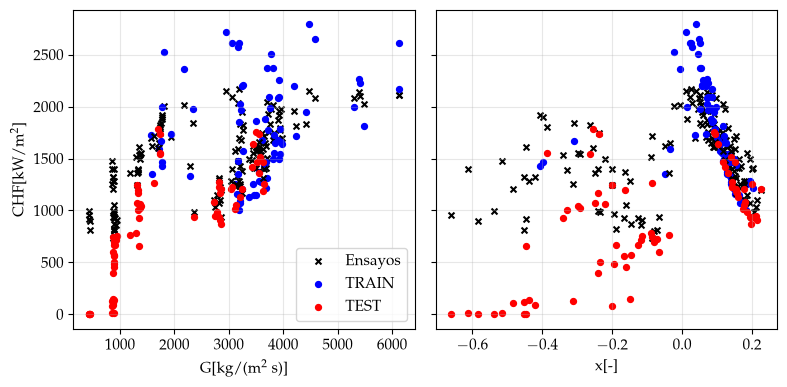
\includegraphics[width=\textwidth]{Figures/chf_lfdnn_gx_caso_mal.png}
    \caption{Relación del CHF predicho con el flujo másico y el título, según el punto predicho por el modelo \texttt{LFDNN} \#4. TRAIN y TEST son los conjuntos de entrenamiento y evaluación correspondientes a la \texttt{HFDNN}, divididos tal que en evaluación se tienen los ensayos de menor flujo másico.}
    \label{fig:lfdnn_chf_gx}
\end{figure}

Para solventar esta dificultad del modelo en la zona subenfriada se propuso una condición de monotonicidad negativa de la derivada del CHF respecto del título termodinámico, es decir, un modelo de PINN para la \lfdnn{}, que se denota \lfpinn{}. Esta incorporación se realizó al modificar el cálculo de la función de pérdida, según la ecuación \ref{eq:lfpinn_loss},
\begin{equation}
    \mathcal{L} = \mathrm{MSE}(\log \mathrm{CHF}) \;+\; \lambda \cdot \frac{1}{\sum w}\sum_i \left[w_i\,\mathrm{ReLU}\!\left(\frac{\partial \log \mathrm{CHF}}{\partial x}\Big|_i\right)\right]^2.
    \label{eq:lfpinn_loss} 
\end{equation}
Los términos $w$ y $w_i$ representan la máscara aplicada por la condición de monotonicidad sobre los puntos de colocación, según en qué región del dominio de las variables de entrada se debe aplicar. En particular, en este caso se diseñó el conjunto de puntos de colocación para la región subenfriada, con valores de presión y $\nicefrac{L}{D_h}$ en los rangos de los ensayos de COBRA3-CP. El término $\lambda$ es el peso atribuido a la condición de monotonicidad. 

\begin{figure}[h]
    \centering
    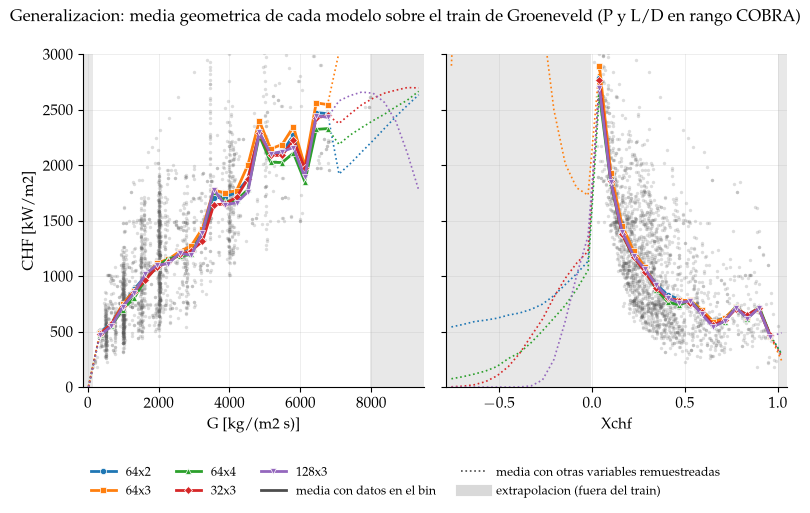
\includegraphics[width=\textwidth]{Figures/chf_lfdnn_generalizacion.png}
    \caption{Evaluación de la generalización de la \lfdnn{} respecto del flujo másico y el título termodinámico.}
    \label{fig:lfdnn_chf_generalizacion}
\end{figure}


Se analizó el impacto de esta implementación en una arquitectura de $64\times 3$, con la misma metodología que las arquitecturas anteriores. Se entrenaron tres redes, variando el valor de $\lambda$ entre $0.01$, $0.1$ y $1$. Esto permite evaluar el impacto del grado en que se impone esta condición frente a los datos.
En la tabla \ref{tab:lfdnn_arqs_comparativa} se presenta la comparativa de las métricas estadísticas sobre los conjuntos de ensayos en un tubo. Esto permite verificar que la condición agregada no perjudica al modelo dentro del conjunto que busca representar.
Se obtiene que los modelos mantienen su precisión respecto de los ensayos de un tubo. La diferencia en RMSE es de menos del $2\%$ respecto del modelo base, lo que indica que la incorporación de la monotonicidad no corrompe el modelo.

\begin{table}[H]
	\centering
	\caption{Arquitecturas de \texttt{LFDNN} propuestas y métricas sobre conjuntos de entrenamiento y evaluación de ensayos en un tubo.}
	\begin{tabular}{c c c c c c} 
        \toprule
        \multirow{2}{*}{\textbf{\#}} & $\bm{\lambda}$ & \multicolumn{2}{c}{$\mathbf{R^2}$} & \multicolumn{2}{c}{\textbf{RMSE}} \\
        & & \textbf{Ent.} & \textbf{Eval.} & \textbf{Ent.} & \textbf{Eval.} \\ \hline
        LUT                     & -      & \multicolumn{2}{c}{$0.898$} & \multicolumn{2}{c}{$507.1$} \\
        Base                    & -      & $0.9657$ & $0.9657$ & $296.1$ & $294.3$ ($+4.2\%$) \\
        \multirow{3}{*}{PINN}   & $0.01$ & $0.9624$ & $0.9642$ & $310.0$ & $300.9$ ($+4.1\%$) \\
                                & $0.1$  & $0.9638$ & $0.9652$ & $304.1$ & $296.8$ ($+4.7\%$) \\
                                & $1$    & $0.9637$ & $0.9650$ & $304.6$ & $297.6$ ($+5.1\%$) \\
		\bottomrule
	\end{tabular}
	\label{tab:lfdnn_arqs_comparativa}
\end{table}

% Groeneveld                --- log CHF ---                  --- CHF [kW/m2] ---        
% modelo             R2 tr   R2 te  RMSE tr  RMSE te   R2 tr   R2 te   RMSE tr   RMSE te
% --------------------------------------------------------------------------------------
% $\lambda$ = 0     0.9665  0.9632   0.1464   0.1530  0.9605  0.9626     317.5     307.4
% $\lambda$ = 0.01  0.9661  0.9630   0.1473   0.1533  0.9624  0.9642     310.0     300.9
% $\lambda$ = 0.1   0.9661  0.9626   0.1473   0.1542  0.9638  0.9652     304.1     296.8
% $\lambda$ = 1     0.9658  0.9620   0.1479   0.1554  0.9637  0.9650     304.6     297.6

% mejor R2 en test (log):   $\lambda$ = 0  (0.9632)
% mejor RMSE en test (log): $\lambda$ = 0  (0.1530)

% brecha train->test (RMSE en log):
%   $\lambda$ = 0    +0.0066 (+4.5%)
%   $\lambda$ = 0.01 +0.0060 (+4.1%)
%   $\lambda$ = 0.1  +0.0069 (+4.7%)
%   $\lambda$ = 1    +0.0076 (+5.1%)

% costo respecto de lambda = 0 (RMSE en log, test):
%   $\lambda$ = 0    +0.00%
%   $\lambda$ = 0.01 +0.20%
%   $\lambda$ = 0.1  +0.80%
%   $\lambda$ = 1    +1.61%


Luego, en la tabla \ref{tab:lfdnn_dnbrmin_comp}, se comparan los valores de media y desvío estándar del DNBR, el $\mathrm{DNBR}_\mathrm{min}$ y los puntos predichos en la región de entrada y en subcanales interiores. Se obtiene una mejora considerable en todos los modelos PINN, lo que indica que la condición aplicada beneficia al modelo en condiciones subenfriadas. Los valores de DNBR quedan prácticamente centrados y su desvío estándar se redujo a la mitad. En cuanto al $\mathrm{DNBR}_\mathrm{min}$, no se obtuvo una mejora, pero esto se debe a su método de cálculo y a la subpredicción no física del DNBR con el modelo base. La cantidad de predicciones en la región de entrada se reduce de casi el $50\%$ de los ensayos a menos del $7\%$. En cuanto a las predicciones en subcanales internos, se obtiene un aumento, aunque se mantiene en menos de $15\%$ de los ensayos. La conclusión es que la aplicación de la monotonicidad mejora la generalización del modelo a la aplicación de interés.

\begin{table}[H]
	\centering
	\caption{Arquitecturas de \texttt{LFDNN} propuestas y métricas sobre ensayos de bundle de la \cna{}.}
	\begin{tabular}{c c c c c c c} 
        \toprule
        \textbf{Arq.} & $\bm{\lambda}$ & $\bm{\overline{\mathrm{DNBR}}}$ & $\bm{\sigma(\mathrm{DNBR})}$ &  $\bm{\mathrm{DNBR}_\mathrm{min}}$ & \textbf{Z entrada} & \textbf{SCH int.} \\ \hline
        Base    & -      & $0.687$ & $0.403$ & $1.442$ & 72 & 6  \\
        \multirow{3}{*}{PINN} 
                & $0.01$ & $1.061$ & $0.219$ & $1.470$ & 10 & 14 \\
                & $0.1$  & $1.035$ & $0.226$ & $1.457$ & 4  & 14 \\
                & $1$    & $1.037$ & $0.224$ & $1.456$ & 3  & 22 \\
		\bottomrule
	\end{tabular}
	\label{tab:lfdnn_dnbrmin_comp}
\end{table}

Se mantuvo el criterio empleado para evaluar la predicción de los modelos base y se graficó la relación del CHF predicho con el flujo másico y el título termodinámico para el modelo \lfpinn{} con $\lambda=0.1$ en la figura \ref{fig:lfdnn_chf_gx_mon}. Se observa que se predicen unos pocos casos de CHF en región subenfriada, lo que indica una mejora considerable del modelo respecto de su versión base. Adicionalmente, no se observan valores de CHF que tiendan a $0$, como en la figura \ref{fig:lfdnn_chf_gx}.
Luego, en la figura \ref{fig:lfdnn_chf_generalizacion_mono}, se presenta la evaluación de la generalización del modelo respecto del flujo másico y el título termodinámico. Se observa que el modelo ahora presenta un aumento del CHF al reducir el título termodinámico en condiciones subenfriadas. Este es el resultado esperado, reforzado por la monotonicidad aplicada. Se observa una reducción del CHF predicho en la región cercana a $x=0$, lo que se debe a los ensayos disponibles en un tubo para condiciones subenfriadas. Se halló que se tienen unos pocos ensayos de un tubo en condiciones subenfriadas, pero con longitud calefaccionada muy por debajo de las de aplicación en este trabajo. Su efecto queda compensado por la condición de monotonicidad y los puntos de colocación durante el entrenamiento. Una posible mejora a futuro es realizar un filtrado del conjunto de ensayos de Groeneveld para que las variables estén en el rango de aplicación final.

\begin{figure}[H]
    \centering
    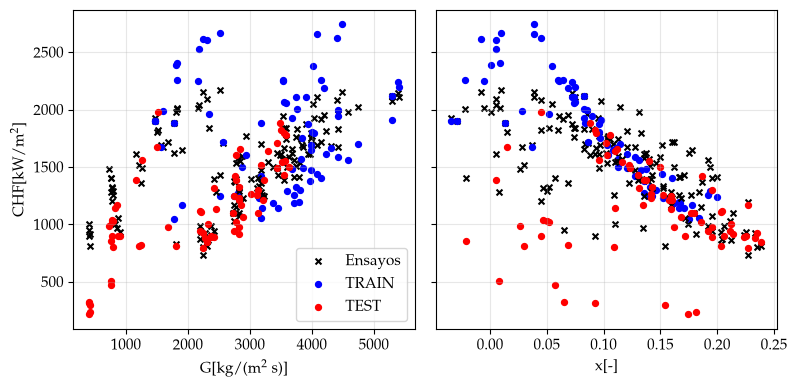
\includegraphics[width=0.9\textwidth]{Figures/chf_lfdnn_gx_mon.png}
    \caption{Relación del CHF predicho con el flujo másico y el título, según el punto predicho por el modelo \texttt{LFDNN} con monotonicidad con $\lambda=0.1$. TRAIN y TEST son los conjuntos de entrenamiento y evaluación correspondientes a la \texttt{HFDNN}, divididos tal que en evaluación se tienen los ensayos de menor flujo másico.}
    \label{fig:lfdnn_chf_gx_mon}
\end{figure}


\begin{figure}[H]
    \centering
    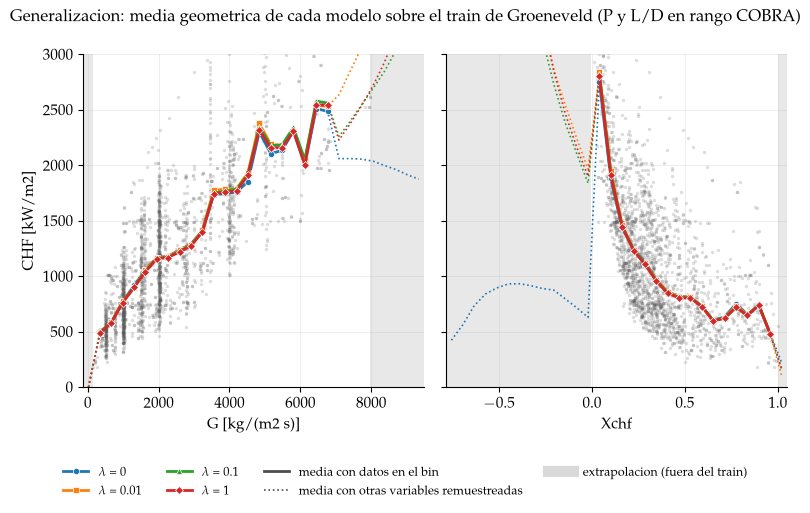
\includegraphics[width=\textwidth]{Figures/chf_lfdnn_generalizacion_mono.png}
    \caption{Evaluación de la generalización de la \lfpinn{} respecto del flujo másico y el título termodinámico, según $\lambda$.}
    \label{fig:lfdnn_chf_generalizacion_mono}
\end{figure}

Por último, en la figura \ref{fig:lfdnn_chf_pred_mono} se grafica el CHF predicho contra medido y el DNBR en cada ensayo para el modelo con $\lambda=0.1$. Se observa una predicción centrada, con algunos outliers en el conjunto de evaluación. Estos casos son los que están por fuera del rango de los ensayos en un tubo, y la red debe extrapolar para estimar CHF. A excepción de estos casos, la predicción del modelo se encuentra contenida en el mismo rango que la metodología actual propuesta por INVAP, que, además de la LUT de Groeneveld, recurre a factores de centrado y corrección desarrollados específicamente para lograr una mejor estimación del CHF en el bundle de la \cna{}, descriptos en la sección \ref{sec:app_tmf}. Esto denota que el modelo de baja fidelidad logra ya una precisión incluso comparable a la metodología actual, sin haber utilizado datos de los ensayos en la geometría específica. 

\begin{figure}[H]
    \centering
    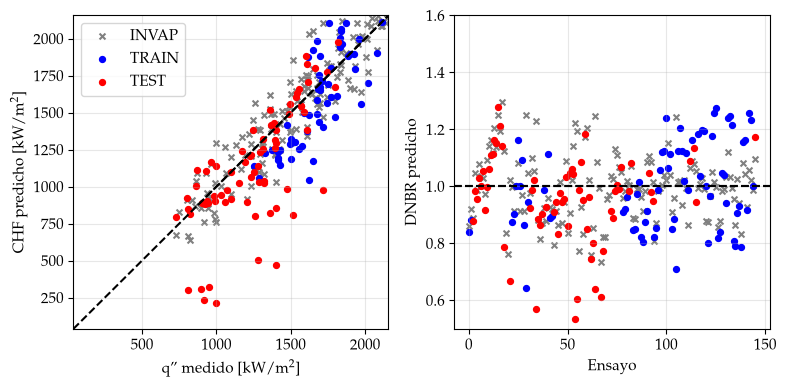
\includegraphics[width=\textwidth]{Figures/chf_lfdnn_pred_mono.png}
    \caption{Predicción de CHF contra medido y $\mathrm{DNBR}$ para cada ensayo, para modelo \lfpinn{} con $\lambda=0.1$.}
    \label{fig:lfdnn_chf_pred_mono}
\end{figure}

Definido el modelo para realizar la estimación de CHF en un tubo, resulta natural la pregunta sobre cómo se compara con la metodología LUT. Para ello, en la figura \ref{fig:lfpinn_lut} se presentan los valores de CHF predicho contra medido para los ensayos de un tubo. Se grafican las predicciones de la LUT y del modelo \lfpinn{} final con $\lambda=0.1$. Gráficamente la mejora es más modesta de lo que el aumento de $\mathrm{R}^2$ y el descenso en RMSE indican. Notar que en la zona de menor CHF se obtiene una sobrepredicción importante del CHF. Esto es producto de la condición de monotonicidad aplicada respecto del título termodinámico. Su efecto es positivo en el contexto de la estimación para el bundle de la \cna{}, pero en el caso general de un tubo no lo es. Como se mencionó previamente, los datos en condiciones subenfriadas se corresponden a ensayos con $\nicefrac{L}{D_h}$ muy lejanos al bundle de \cna{}, por lo que su exclusión para el entrenamiento de la \lfpinn{} sería recomendable.

En la bibliografía se han realizado modelos basados en Machine Learning que han obtenido mejor rendimiento que la \lfpinn{}. Aún así, el objetivo del modelo en el contexto de este trabajo es tener una predicción confiable del CHF en un tubo como primer aproximación. La optimización del modelo \lfpinn{} no se realizó de forma rigurosa y en función de lo informado en la tabla \ref{tab:lfdnn_arqs} se evidencia un margen de mejora con redes más densas.

\begin{figure}[H]
    \centering
    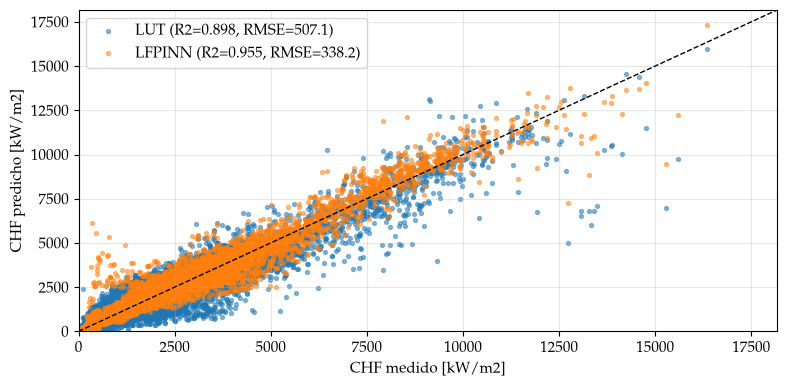
\includegraphics[width=\textwidth]{Figures/lfpinn_lut.png}
    \caption{Predicción de CHF contra medido para \lfpinn{} y LUT.}
    \label{fig:lfpinn_lut}
\end{figure}

\section{Análisis de arquitectura informada por física}
\label{app_chf_mfpinn}
En esta sección se presentan los resultados complementarios del análisis de arquitectura informada por física, discutido en la sección \ref{sec:chf_arq_mfpinn} del capítulo \ref{Chapter4}. La tabla \ref{tab:mfpinn_arqs_dnbr_train} presenta los resultados de predicción de DNBR sobre el conjunto de entrenamiento para las variantes de \mfpinn{} descriptas en la tabla \ref{tab:mfpinn_arqs}. Las figuras \ref{fig:chf_pred_mfpinn_a}, \ref{fig:chf_pred_mfpinn_b} y \ref{fig:chf_pred_mfpinn_d} presentan el CHF predicho contra medido y el DNBR por ensayo para las variantes A, B y D, respectivamente. Por último, las figuras \ref{fig:chf_gx_mfpinn_a}, \ref{fig:chf_gx_mfpinn_b} y \ref{fig:chf_gx_mfpinn_d} muestran la relación entre el CHF predicho y el flujo másico y el título termodinámico para las mismas variantes.

\begin{table}[H]
	\centering
	\caption{Resultados de predicción de CHF sobre conjunto de entrenamiento para las arquitecturas evaluadas de \mfpinn{}.}
	\begin{tabular}{c c c c c} 
        \toprule
        \textbf{Modelo} & $f_c$ & $\overline{\mathrm{DNBR}}$ & $\sigma(\mathrm{DNBR})$ & $\mathrm{DNBR}_\mathrm{min}$ \\ \hline
        \mfdnn{}& $1.000$
                                        & $1.000$ & $0.032$ & $1.062$ \\
        A       & $1.000$
                                        & $1.000$ & $0.019$ & $1.037$ \\
        B       & $1.000$
                                        & $1.000$ & $0.021$ & $1.041$ \\
        B1      & $1.000$
                                        & $1.000$ & $0.021$ & $1.042$ \\
        B2      & $1.000$
                                        & $1.000$ & $0.020$ & $1.040$ \\
        B3      & $1.000$
                                        & $1.000$ & $0.023$ & $1.044$ \\
        C       & $1.000$
                                        & $1.000$ & $0.019$ & $1.038$ \\
        D       & $1.000$
                                        & $1.000$ & $0.022$ & $1.044$ \\
        E       & $1.000$
                                        & $1.000$ & $0.020$ & $1.039$ \\
		\bottomrule
	\end{tabular}
	\label{tab:mfpinn_arqs_dnbr_train}
\end{table}


\begin{figure}[H]
    \centering
    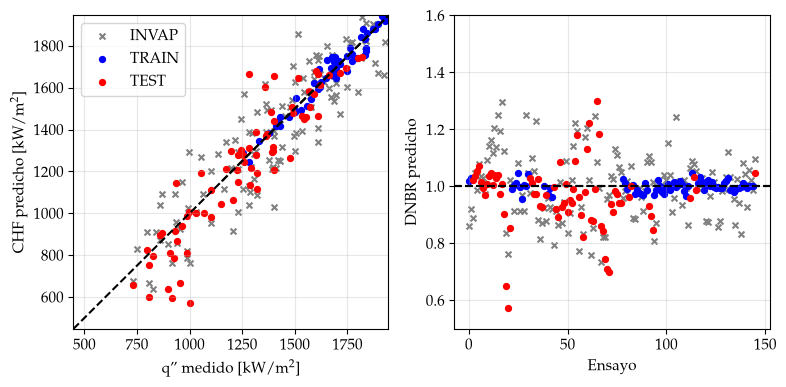
\includegraphics[width=0.95\textwidth]{Figures/chf_mfpinn_A.png}
    \caption{CHF predicho contra medido y DNBR por ensayo para variante A de \mfpinn{}.}
    \label{fig:chf_pred_mfpinn_a}
\end{figure}

\begin{figure}[H]
    \centering
    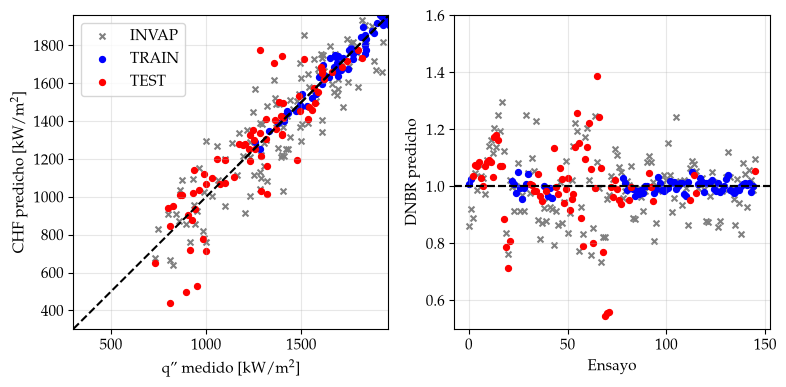
\includegraphics[width=0.95\textwidth]{Figures/chf_mfpinn_B.png}
    \caption{CHF predicho contra medido y DNBR por ensayo para variante B de \mfpinn{}.}
    \label{fig:chf_pred_mfpinn_b}
\end{figure}

\begin{figure}[H]
    \centering
    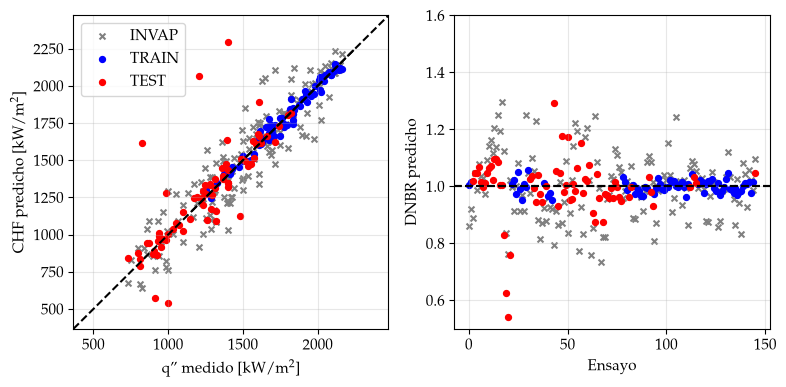
\includegraphics[width=0.95\textwidth]{Figures/chf_mfpinn_D.png}
    \caption{CHF predicho contra medido y DNBR por ensayo para variante D de \mfpinn{}.}
    \label{fig:chf_pred_mfpinn_d}
\end{figure}

\begin{figure}[H]
    \centering
    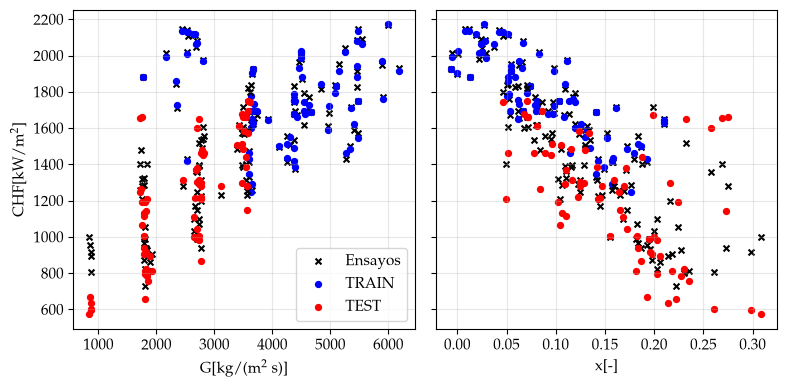
\includegraphics[width=0.95\textwidth]{Figures/chf_mfpinn_gx_A.png}
    \caption{Relación entre CHF predicho y flujo másico y título termodinámico para variante A de \mfpinn{}.}
    \label{fig:chf_gx_mfpinn_a}
\end{figure}

\begin{figure}[H]
    \centering
    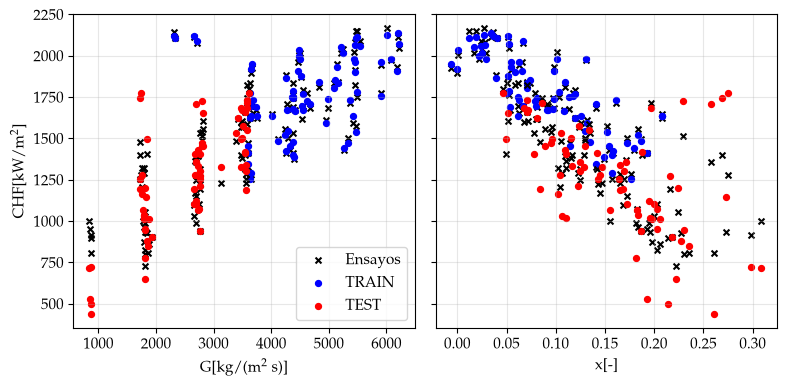
\includegraphics[width=0.95\textwidth]{Figures/chf_mfpinn_gx_B.png}
    \caption{Relación entre CHF predicho y flujo másico y título termodinámico para variante B de \mfpinn{}.}
    \label{fig:chf_gx_mfpinn_b}
\end{figure}

\begin{figure}[H]
    \centering
    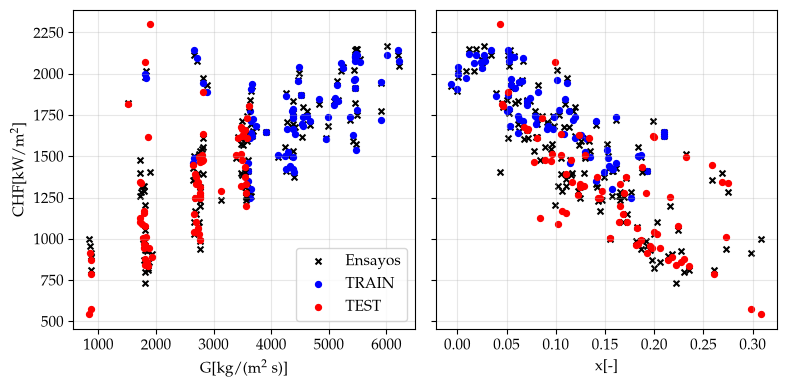
\includegraphics[width=0.95\textwidth]{Figures/chf_mfpinn_gx_D.png}
    \caption{Relación entre CHF predicho y flujo másico y título termodinámico para variante D de \mfpinn{}.}
    \label{fig:chf_gx_mfpinn_d}
\end{figure}

\subsection{Análisis de variables de entrada}
\label{sec:chf_variables_entrada}

Las variables de entrada propuestas en la sección \ref{sec:chf_pipeline} fueron el flujo másico, la presión, el título termodinámico, la relación de largo calefaccionado con diámetro hidráulico, la distancia adimensional al separador aguas arriba, el desbalance de título termodinámico respecto del valor medio del bundle, el factor de pico de potencia y la relación entre perímetro calefaccionado y mojado del subcanal. 
Las primeras cuatro variables son las clásicas utilizadas por la LUT de Groeneveld, y se consideran las más importantes para la predicción de CHF. Las cuatro variables restantes fueron propuestas en este trabajo, y se debe evaluar su contribución al modelo.

Se entrenaron el modelo \mfdnn{} y las variantes A, B, C y D del modelo \mfpinn{}. Al igual que en la sección anterior, para el modelo \mfdnn{} se entrenaron 50 instancias y se informan las medianas de las métricas. En cuanto a las variantes \mfpinn{}, no se realizó un estudio de ese tipo, debido a que su costo de entrenamiento es considerablemente elevado.

En la tabla \ref{tab:mfpinn_exp_dnbr_train} se presentan el factor de centrado, la media y el desvío estándar del DNBR predicho y el \dnbrmin{} para el conjunto de entrenamiento. Se obtuvo un rendimiento similar al del caso con las variables base, levemente mejorado en las variantes \mfpinn{}.

\begin{table}[H]
	\centering
	\caption{Resultados de predicción de CHF sobre conjunto de entrenamiento para las arquitecturas evaluadas de \mfpinn{}.}
	\begin{tabular}{c c c c c} 
        \toprule
        \textbf{Modelo} & $f_c$ & $\overline{\mathrm{DNBR}}$ & $\sigma(\mathrm{DNBR})$ & $\mathrm{DNBR}_\mathrm{min}$ \\ \hline
        \mfdnn{}    & $1.007$ & $1.000$ & $0.028$ & $1.055$ \\
        \mfpinn{} A & $1.000$ & $1.000$ & $0.010$ & $1.020$ \\
        \mfpinn{} B & $1.000$ & $1.000$ & $0.014$ & $1.028$ \\
        \mfpinn{} D & $1.000$ & $1.000$ & $0.018$ & $1.035$ \\
        \mfpinn{} E & $1.000$ & $1.000$ & $0.013$ & $1.026$ \\
		\bottomrule
	\end{tabular}
	\label{tab:mfpinn_exp_dnbr_train}
\end{table}

En cuanto al conjunto de evaluación, sí se obtuvieron diferencias en el rendimiento respecto de utilizar las variables base. En la tabla \ref{tab:mfpinn_exp_dnbr_test} se presentan las métricas para dicho conjunto. La \mfdnn{} presenta un rendimiento casi idéntico al caso anterior. Las variantes A y E de \mfpinn{} presentaron un rendimiento muy pobre, con un \dnbrmin{} mayor incluso que el de la \lfdnn{}. La variante B presenta una mejora, producto de una reducción del desvío estándar y un aumento en la subpredicción del CHF. 
La variante D presenta un rendimiento sobresaliente, con el mejor \dnbrmin{} obtenido hasta este punto del trabajo. Por ello, se investigó el resultado con mayor detalle, al graficar la relación de los CHF predichos con el flujo másico y el título termodinámico en la figura \ref{fig:chf_mfpinn_d_gx_exp}. Allí se puede ver que el modelo predice CHF en condiciones subenfriadas en múltiples ensayos. Este resultado pone en tela de juicio el sentido físico de estas predicciones.

\begin{table}[H]
	\centering
	\caption{Resultados de predicción de CHF sobre conjunto de evaluación para las arquitecturas evaluadas de \mfpinn{}.}
	\begin{tabular}{c c c c c} 
        \toprule
        \textbf{Modelo} & $f_c$ & $\overline{\mathrm{DNBR}}$ & $\sigma(\mathrm{DNBR})$ & $\mathrm{DNBR}_\mathrm{min}$ \\ \hline
        \mfdnn{}    & $1.007$ & $1.046$ & $0.097$ & $1.238$ \\
        \mfpinn{} A & $1.000$ & $1.233$ & $0.451$ & $2.125$ \\
        \mfpinn{} B & $1.000$ & $0.953$ & $0.126$ & $1.202$  \\
        \mfpinn{} D & $1.000$ & $0.956$ & $0.089$ & $1.133$  \\
        \mfpinn{} E & $1.000$ & $1.321$ & $0.358$ & $2.030$  \\
		\bottomrule
	\end{tabular}
	\label{tab:mfpinn_exp_dnbr_test}
\end{table}

\begin{figure}[H]
    \centering
    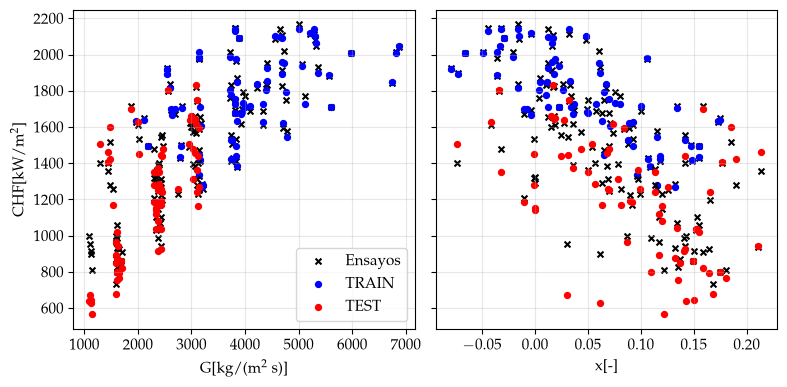
\includegraphics[width=0.95\textwidth]{Figures/chf_mfpinn_gx_D_exp.png}
    \caption{Relación de CHF con el flujo másico y el título termodinámico para variante D de \mfpinn{}, con variables de entrada expandidas.}
    \label{fig:chf_mfpinn_d_gx_exp}
\end{figure}

Se presentan los resultados de CHF predicho contra real y DNBR por ensayo para el modelo \mfdnn{} en la figura \ref{fig:chf_mfdnn_exp} y para la variante E del modelo \mfpinn{} en la figura \ref{fig:chf_mfpinn_exp}. Ambos obtienen una tendencia a la sobrepredicción para el conjunto de evaluación. Para la variante E se observa un rendimiento muy pobre, como lo indican las métricas de DNBR, con una sobrepredicción preocupante del CHF.

\begin{figure}[H]
    \centering
    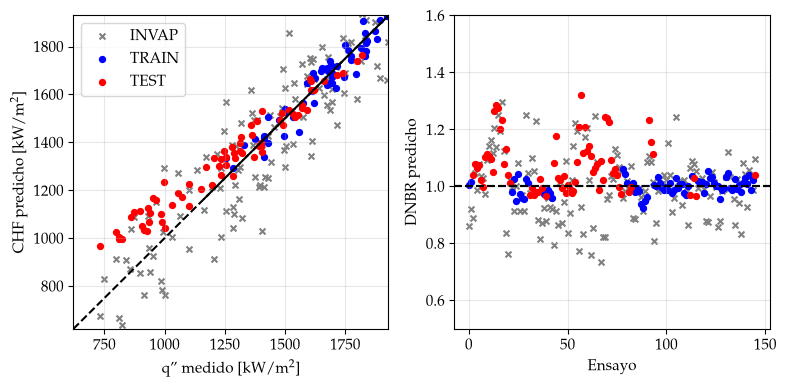
\includegraphics[width=0.95\textwidth]{Figures/chf_mfdnn_pred_exp.png}
    \caption{CHF predicho contra real y DNBR por ensayo, para \mfdnn{} con variables de entrada expandidas.}
    \label{fig:chf_mfdnn_exp}
\end{figure}

\begin{figure}[H]
    \centering
    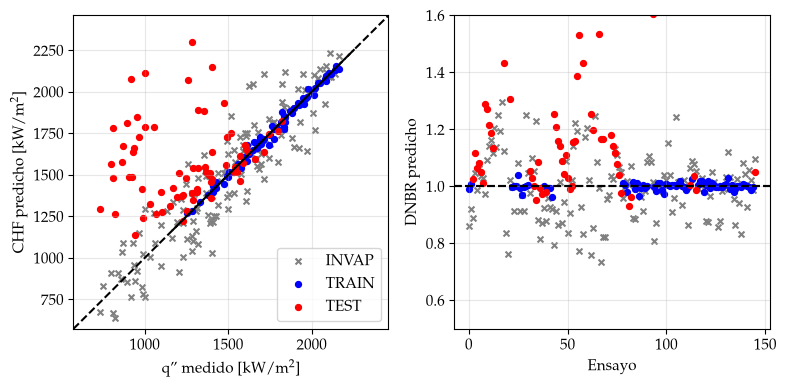
\includegraphics[width=0.95\textwidth]{Figures/chf_mfpinn_E_exp.png}
    \caption{CHF predicho contra real y DNBR por ensayo, para variante E de \mfpinn{} con variables de entrada expandidas.}
    \label{fig:chf_mfpinn_exp}
\end{figure}

La conclusión obtenida es que la inclusión de estas variables en el modelo no representa una mejora clara en las predicciones, e incluso puede resultar en predicciones con tendencias no físicas. Por lo tanto, los modelos finales solo utilizan las variables básicas.

\section{Modelo final}
En la figura \ref{fig:dist_mfdnn_final} se presenta la distribución de densidad de probabilidad de \dnbrmin{} para los 50 modelos \mfdnn{} entrenados, resultado discutido en la sección \ref{sec:chf_modelos_finales} del capítulo \ref{Chapter4}.

\begin{figure}[H]
    \centering
    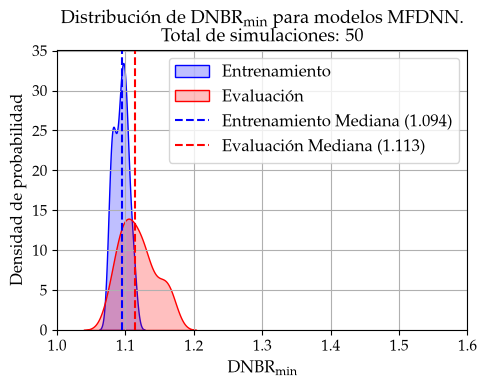
\includegraphics[width=0.6\textwidth]{Figures/chf_distribucion_mfdnn_final.png}
    \caption{Distribución de densidad de probabilidad de \dnbrmin{} para 50 modelos \mfdnn{} entrenados.}
    \label{fig:dist_mfdnn_final}
\end{figure}